\section{Mengen, Relationen und Abbildungen}
  \begin{definition}
    Mengen sind Ansammlungen von Elementen.
  \end{definition}
  \subsection{Arten von Mengen}
	  \begin{figure}[htbp] 
		  \centering
		  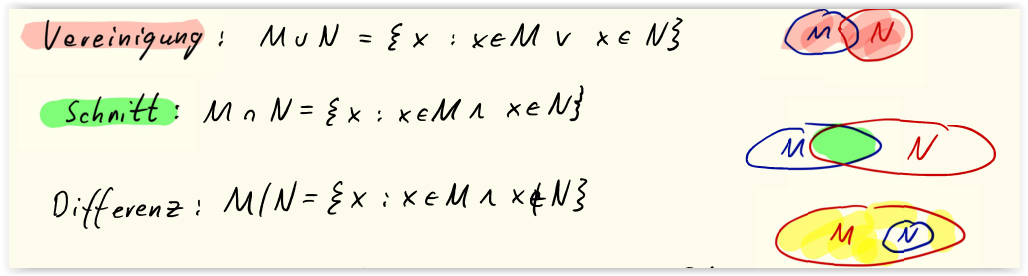
\includegraphics[width=0.9\textwidth]{./img/mengen_arten.png}
		  \caption{Arten von Mengen\protect\cite{HM12}}
		  \label{fig:mengen_arten}
		\end{figure}
	  \begin{definition}
	    Ist $N \subset M$ dann heißt $N^c = M/N$ das Komplement von $N$. $M$ und $N$ heißen disjunkt, falls $M \cap N = \mathcal{O}$, wobei $\mathcal{O} = \lbrace \rbrace$ die leere Menge ist.
	  \end{definition}
	  \begin{definition}
	    Kartesisches Produkt: $M \times N = \lbrace (a,b): a \in M \land b \in N\rbrace$
	  \end{definition}
	  \begin{definition}
	    Potenzmenge: $P(M) = \lbrace X:X\subset M\rbrace$
	  \end{definition}
	  \subsubsection{Abkürzungen}
	  \begin{itemize}
	    \item $\bigcup\limits_{k = 1}^n A_k = A_1 \cup ... \cup A_n$
	    \item $\bigcap\limits_{k=1}^n A_k = A_1 \cap ... \cap A_n$
	    \item $\prod\limits_{k=1}^n A_k = A_1 \times ... \times A_n = \lbrace \underbrace{(a_1, ..., a_n)}_{n-Tupel}:\forall k: a_k \in A_k \rbrace$
	  \end{itemize}
	\subsection{Relationen}
	\begin{definition}
	  Relationen setzen Elemente zweier Mengen in Verbindung. Eine Relatiopn ist eine Teilmenge $R\subset M \times N$ mit $M$ und $N$ als Mengen. Man schreibt:
	  \begin{equation*}
	    xRy \text{ genau dann wenn } (x,y) \in R\subset M\times N
	  \end{equation*}
	  Jede Funktion $f \rightarrow f(x)$ ist eine Relation $R=\lbrace (x, f(x)): x\in \R \rbrace \subset \R \times \R$.
	\end{definition}
	\subsubsection{Äquivalenzrelationen}
	  Eigenschaften:
	  \begin{itemize}
	    \item $aRa$, d.h. $(a,a) \in R$ \colBlue{(Reflexivität)}
	    \item $aRb \Leftrightarrow bRa$, d.h. mit $(a,b)\in R$ ist auch $(b,a) \in R$ \colBlue{(Symmetrie)}
	    \item $aRb \land bRc \Rightarrow aRc$, d.h. mit $(a,b) \in R$ und $(b,c) \in R$ ist auch $(a,c) \in R$ \colBlue{(Transitivität)}
	  \end{itemize}
	  \begin{satz}
	    Ist $R$ eine Äquivalenzrelation, d.h. eine Relation mit obigen Eigenschaften, so zerfällt die Menge $M$ in disjunkte Teilmengen. \newline
	    Beispiel:
	    \begin{align*}
	      M &= \lbrace 1,2,3,4\rbrace \\
	      R &= \lbrace(1,3),(3,1),(1,1),(3,3),(2,4),(4,2),(2,2),(4,4)\rbrace\\
	      &\text{$R$ zerlegt $M$ in zwei Klassen (Teilmengen:}\\
	      \lbrace 2,4\rbrace &= [2]_R = [4]_R\\
	      \lbrace 1,3\rbrace &= \underbrace{[1]_R = [3]_R}_{\text{\parbox{2cm}{\centering% 
Repräsentanten \\[-1ex]der Klasse}}}
	    \end{align*}
	    bzw. allgemein: Äquivalenzklasse zu einem Element $a$ bezüglioch einer Äquivalenzrelation $R$
	    \begin{equation*}
	      [a]_R = \lbrace b \in M : aRb\rbrace
	    \end{equation*}
	    Die Menge aller Äquivalenzklassen ist: $M/_R = \lbrace[a]_R: a\in M\rbrace$. Es gilt entweder $[a]_R = [b]_R$ oder $[a]_R \cap [b]_R = \mathcal{O}$.
	  \end{satz}
	  \begin{bem}
	    Es wird häufig anstatt $R$ das Zeichen $\sim$ verwendet.
	  \end{bem}
	\subsubsection{Ordnungsrelationen}
	\begin{definition}
	  Eine Halbordnung $R\subset M \times M$ auf einer Menge $M$ erfüllt
	  \begin{itemize}
	    \item[(i)]   $xRx$
	    \item[(ii)]  $xRy \land yRx \Rightarrow y=x$
	    \item[(iii)] $xRy \land <Rz \Rightarrow xRz$ \colBlue{(Transitivität)}
	  \end{itemize}
	\end{definition}
	\begin{definition}
	  Ordnungsaxiome im $\R$
	  \begin{itemize}
	    \item[(i)]   $x \leq x$
	    \item[(ii)]  $x \leq y \land y \leq x \Rightarrow y = x$
	    \item[(iii)] $x \leq y \land y \leq z \Rightarrow x \leq z$
	    \item[(iv)] $x \leq y \lor y \leq x$ \colBlue{(Totalordnung)}
	    \item[(v)] $x \Rightarrow x+z \leq y+z$ \colBlue{(Zusammenhang mit Addition)}
	    \item[(vi)] $x\leq y \land z \geq 0 \Rightarrow x \cdot z \leq y \cdot z$ \colBlue{(Zusammenhang mit Multiplikation)}
	  \end{itemize}
	\end{definition}
	\begin{definition}
		Zu $a \in \R$ heißt
		\begin{align}
		  |a|:= 
		  \begin{cases} 
		    &a\quad ,\;falls\;a\geq 0 \\ -&a\quad ,\;falls \; a < 0 
		  \end{cases}
		\end{align}
		der Betrag von $a$.
	\end{definition}
	\subsection{Maximum, Minimum, Supremum, Infimum}
	Im Folgenden sei $M$ eine Teilmenge von $\R$.
	\begin{definition}
	  $x \in \R$ heißt eine obere Schranke von $M$, falls $y \leq x$ für alle $y \in M$ gilt. 
	\end{definition}
	\begin{definition}
	  $x \in \R$ heißt eine untere Schranke von $M$, falls $y \geq x$ für alle $y \in M$ gilt. 
	\end{definition}
	\begin{definition}
	  $M$ heißt beschränkt, falls $M$ nach oben und unten beschränkt ist, d.h. eine obere und eine untere Schranke existieren.
	\end{definition}
	\begin{definition}
	  $s = \sup M \in \R$ heißt das Supremum von $M$ und ist die kleinste obere Schranke, d.h. falls $s$ eine obere Schranke von $M$ ist und ferner jede andere obere Schranke $x$ von $M$ die Ungleichung $x\geq s$ erfüllt.
	\end{definition}
	\begin{definition}$\;$\newline
    \vspace{-0.7cm}
	  \begin{itemize}
	    \item[] Infimum: $\inf M \in \R$ ist die größte untere Schranke
	    \item[] Maximum: $s = \max M \in \R$ heißt das Maximum von $M$, falls $s \in M$ und für alle $x \in M$ gilt: $x\leq s$.
	    \item[] Minimum: $s = \min M \in \R$ heißt das Minimum von $M$, falls $s \in M$ und für alle $x \in M$ gilt: $s \leq x$.
	  \end{itemize}
	\end{definition}
	\begin{bem}
	  Für jede endliche Menge existiert das Maximum und Minimum.
	\end{bem}
	\begin{satz}
	  Jede nicht leere, nach oben beschränkte Menge $M \subset \R$ besitzt ein Supremum. (Analog jede nach unten beschränkte Menge ein Infimum)
	\end{satz}
	\begin{bem}
	  \begin{align}
	    \sup(T) \in T &\Rightarrow \sup(T) = \max(T) \\
	    \inf(T) \in T &\Rightarrow \inf(T) = \min(T)
	  \end{align}
	\end{bem}
	\subsection{Abbildungen}
	Abbildungen sind spezielle Relationen. Eine Abbildung $f$ von einer Menge $M$ in eine Menge $N$ ist eine Vorschrift, die jedem $x \in M$ genau ein $y \in N$ zuordnet. $M$ heißt der Definitionsbereich und $N$ heißt der Bildbereich. 
	\begin{definition}
	  $f: M\rightarrow N$ heißt surjektiv, falls die Gleichung $f(x) = y$ mindestens eine Lösung besitzt und zwar für alle $y \in N$.\newline
	  $f:M\rightarrow N$ heißt injektiv, falls für alle $x_1, x_2 \in M: f(x_1) = f(x_2) \Rightarrow x_1 = x_2$.\newline
	  $f$ heißt bijektiv, falls $f$ sowohl injektiv, als auch surjektiv ist.
	\end{definition}
	\subsection{Unendlichkeit}
	\begin{definition}
	  Eine Menge $M$ heißt endlich, falls es ein $n \in N$ und eine bijektive Abbildung $\Phi: \lbrace 1,...,n\rbrace \rightarrow M$ gibt. Eine Menge $M$ heißt abzählbar, falls es eine bijektive Abbildung $\Phi: \N \rightarrow M$ gibt. Sonst heißt die Menge überabzählbar.
	\end{definition}
	\begin{satz}
	  Die Menge der rationalen Zahlen $\Q$ ist abzählbar.
	\end{satz}
	\begin{satz}
	  Die reelen Zahlen sind überabzählbar.
	\end{satz}
	
	\subsection{Elementare realwertige Funktionen}
	  \subsubsection{Algebraische Funktionen}
	  Durch arithmetische Operationen aufgebaut (+,-,$\cdot$,$\backslash$), z.B.: \newline $f(x) = x^2 + 5x$, $f(x) = \sqrt[3]{x}$
    \subsubsubsection{Polynome (+,-,$\cdot$)}
    \begin{equation}
      y = f(x) = a_n x^n + a_{n-1} x^{n-1} + ... + a_0,\quad a_j \in \R
    \end{equation}  
		\vspace{-0.7cm}  	  
	  \begin{figure}[H] 
		\centering
		\begin{minipage}{.5\textwidth}
		  \centering
		  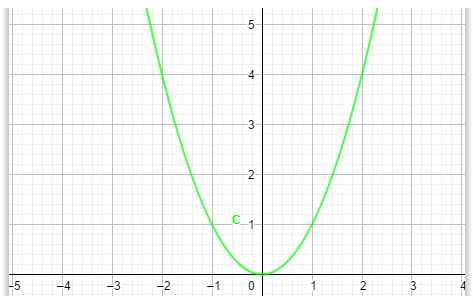
\includegraphics[width=0.7\linewidth]{./img/funktionen_quadratisch.png}
		  \caption{$y = x^2\quad (vgl.\; x^4, x^6, ...)$}
		  \label{fig:funkt_quadr}
		\end{minipage}%
		\begin{minipage}{.5\textwidth}
		  \centering
		  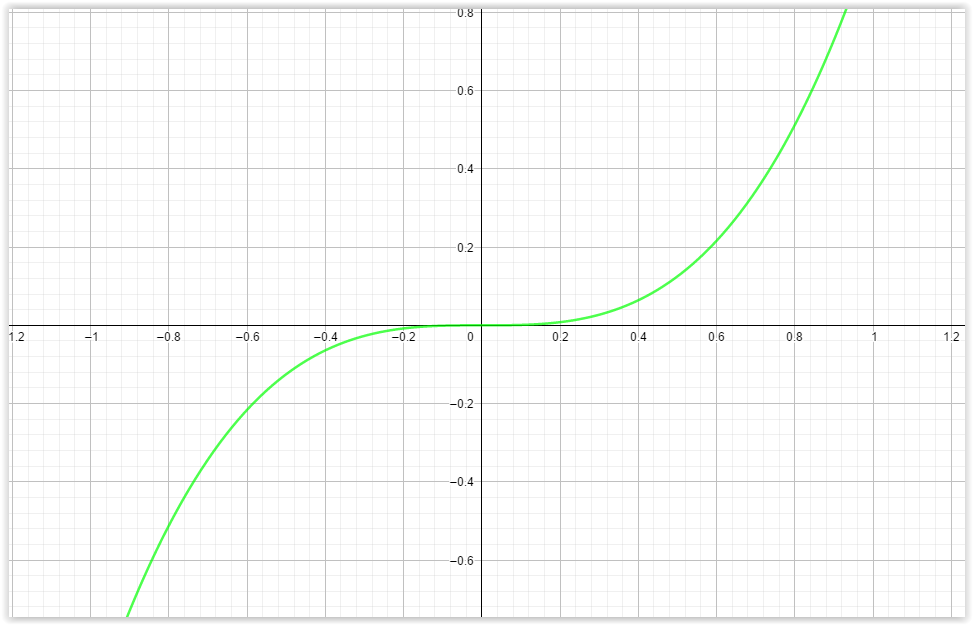
\includegraphics[width=0.7\linewidth]{./img/funktionen_kubisch.png}
		  \caption{$y = x^3 \quad (vgl.\;x^5, x^7, ...)$}
		  \label{fig:funkt_kub}
		\end{minipage}
		\end{figure}
		\vspace{-0.5cm}
		\begin{figure}[H]
		  \centering
		  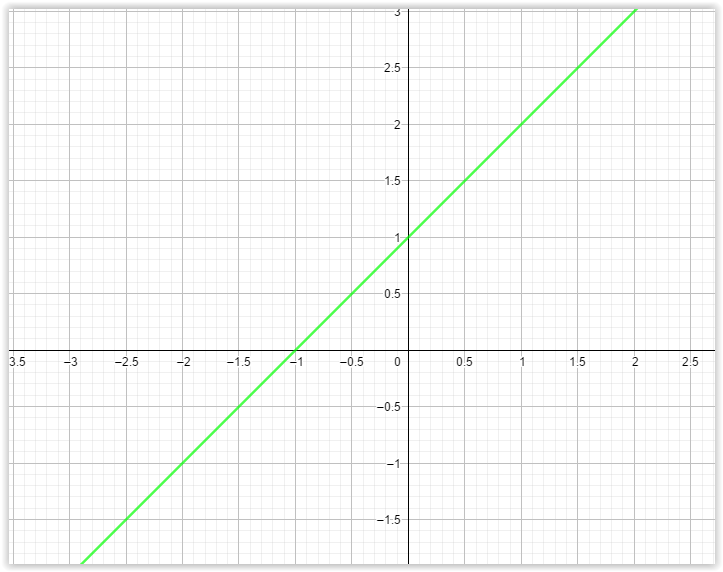
\includegraphics[width=0.3\linewidth]{./img/funktionen_linear.png}
		  \caption{$y = ax+b$}
		  \label{fig:funkt_lin}
		\end{figure}
		
		\vspace{-0.5cm}
		\newpage
		\subsubsubsection{Rationale Funktionen (+,-,$\cdot$, $\backslash$)}
		\begin{equation}
		  y = f(x) = \frac{p(x)}{q(x)} \qquad \text{mit } p,q \text{ sind Polynome}
		\end{equation}
		\begin{figure}[H] 
		\centering
		\begin{minipage}{.5\textwidth}
		  \centering
		  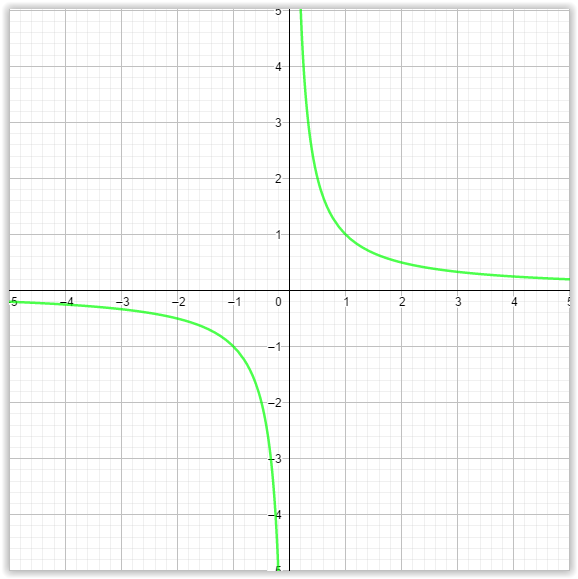
\includegraphics[width=0.6\linewidth]{./img/funktionen_pole_1.png}
		  \caption{$y = \frac{1}{x}$}
		  \label{fig:funkt_pole_1}
		\end{minipage}%
		\begin{minipage}{.5\textwidth}
		  \centering
		  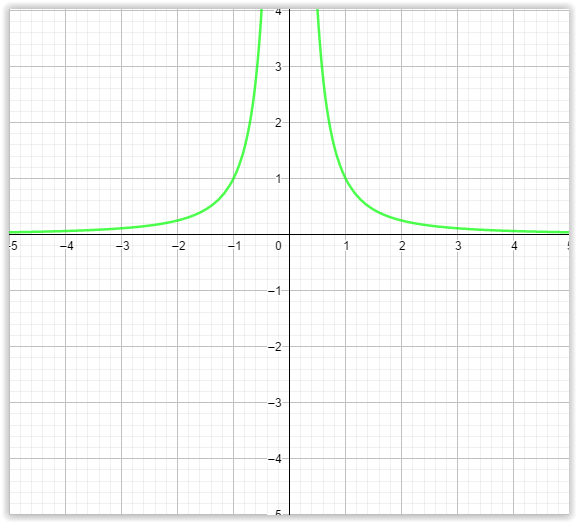
\includegraphics[width=0.65\linewidth]{./img/funktionen_pole_2.png}
		  \caption{$y = \frac{1}{x^2}$}
		  \label{fig:funkt_pole_2}
		\end{minipage}
		\end{figure}
		
		\subsubsubsection{n-te Wurzel}
		\begin{equation}
		  y = f(x) = \sqrt[n]{x}
		\end{equation}
		\begin{figure}[H] 
		\centering
		\begin{minipage}{.5\textwidth}
		  \centering
		  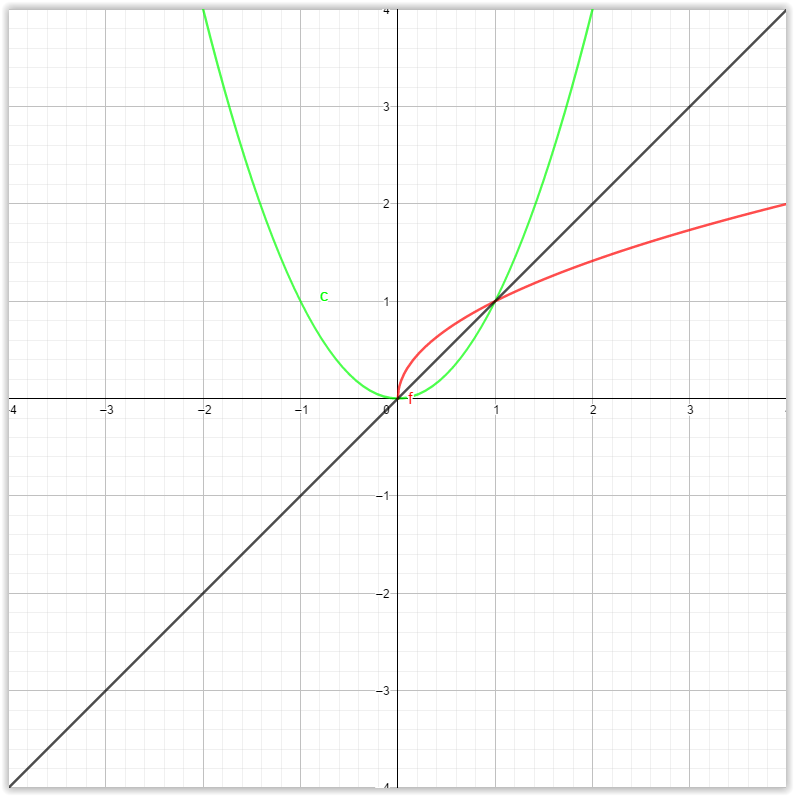
\includegraphics[width=0.6\linewidth]{./img/funktionen_wurzel_2.png}
		  \caption{Quadratwurzel}
		  \label{fig:funkt_root_1}
		\end{minipage}%
		\begin{minipage}{.5\textwidth}
		  \centering
		  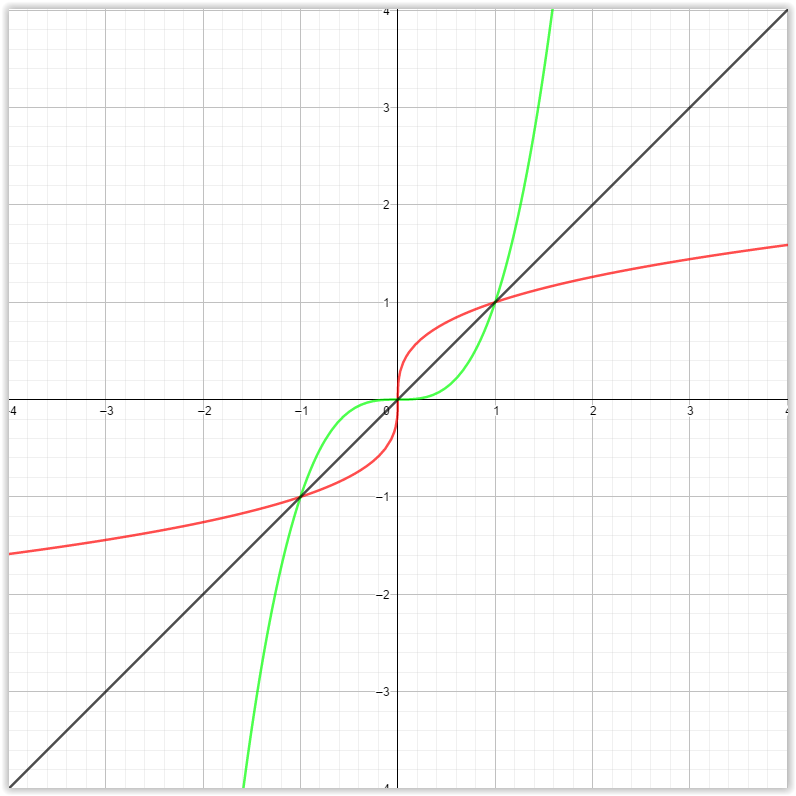
\includegraphics[width=0.6\linewidth]{./img/funktionen_wurzel_3.png}
		  \caption{Kubische Wurzel}
		  \label{fig:funkt_root_2}
		\end{minipage}
		\end{figure}
		Wie man an den Graphiken erkennt ist die Wurzel gerade die Spiegelung an der Ursprungsgeraden des korrelierenden Polynoms. 
		
		\subsubsection{Transzendentale Funktionen}
		\subsubsubsection{Exponentialfunktionen}
		\begin{equation}
		  y =? f(x) = e^x \qquad, e = 2,7182...
		\end{equation}
		Streng monoton wachsende Funktion. Es gilt:
		\begin{equation}
		  \lim_{x\rightarrow \infty} e^x = \infty \qquad \lim_{x\rightarrow -\infty} e^x = 0
		\end{equation}
		
		\subsubsubsection{Unendliche Summen}
		Zum Beispiel Taylorreihen, Potenzreihen
		
		\subsubsubsection{(Natürlicher) Logarithmus}
		\begin{equation}
		  y = f(x) = ln(x)
		\end{equation}
		Bildet das Inverse der e-Funktion. 
		\begin{figure}[H]
		  \centering
		  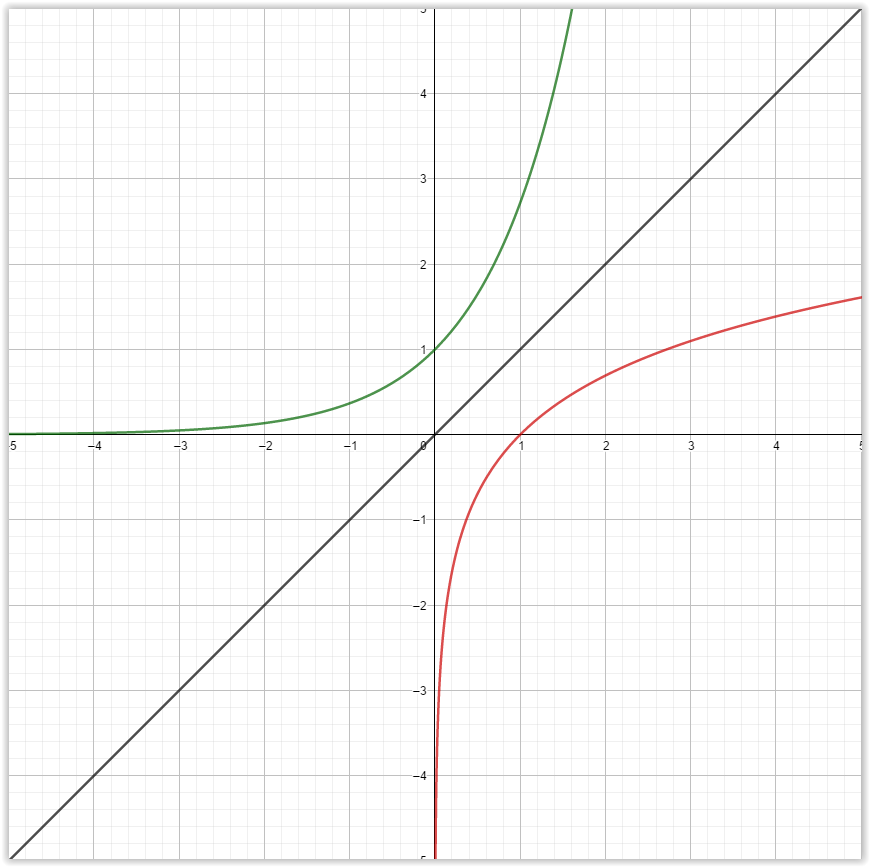
\includegraphics[width=0.35\linewidth]{./img/funktionen_e_ln.png}
		  \caption{Grün: $y = e^x$; Rot: $y = ln(x)$}
		  \label{fig:funkt_e_ln}
		\end{figure}
		Zum Wechsel der Basis können die Logarithmusgesetze angewandt werden:
		\begin{align}
		  h(x) &= a^x = e^{x \cdot ln(x)} \text{, da } ln(a^x) = x\;ln(a) \nonumber \\
		  k(x) &= log_a(x) = \frac{ln(x)}{ln(a)}
		\end{align}
		
		\subsubsubsection{Trigonometrische Funktionen}
		\begin{figure}[H]
		  \centering
		  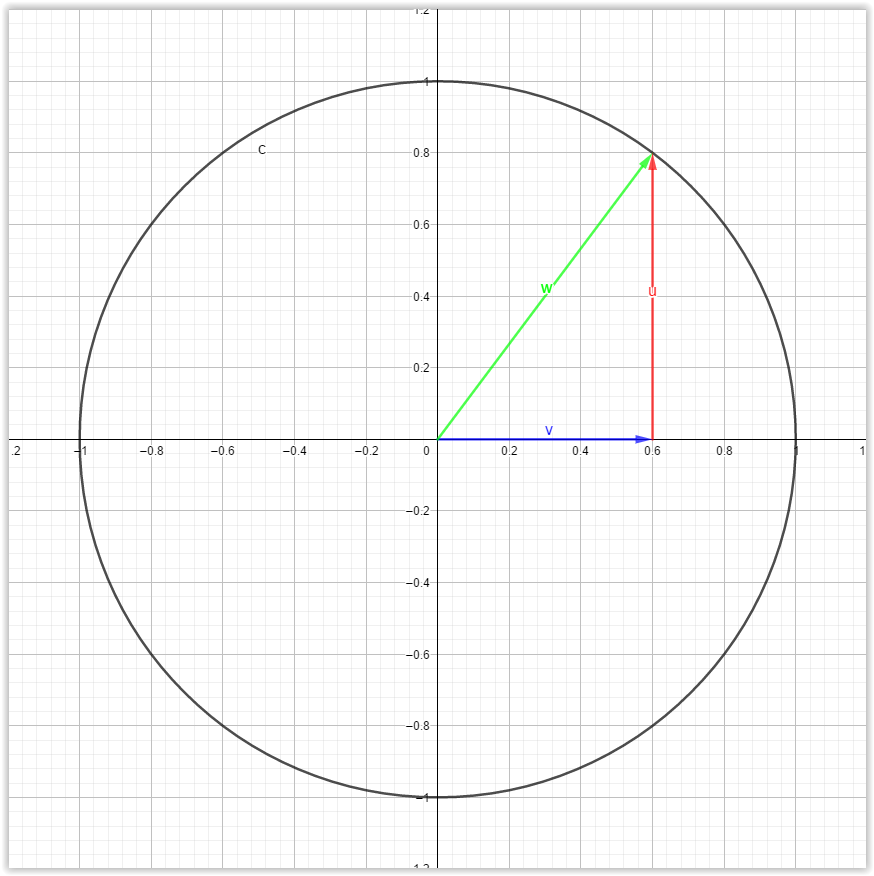
\includegraphics[width=0.35\linewidth]{./img/funktionen_einheitskreis_sin_cos.png}
		  \caption{Grün: $1$; Rot: $sin(x)$; Blau: $cos(x)$}
		  \label{fig:funkt_e_ln}
		\end{figure}
		Aus dem Einheitskreis geht die Identität
		\begin{equation}
		  sin^2(x) + cos^2(x) = 1
		\end{equation}
		direkt hervor.
		\begin{figure}[H] 
		\centering
		\begin{minipage}{.5\textwidth}
		  \centering
		  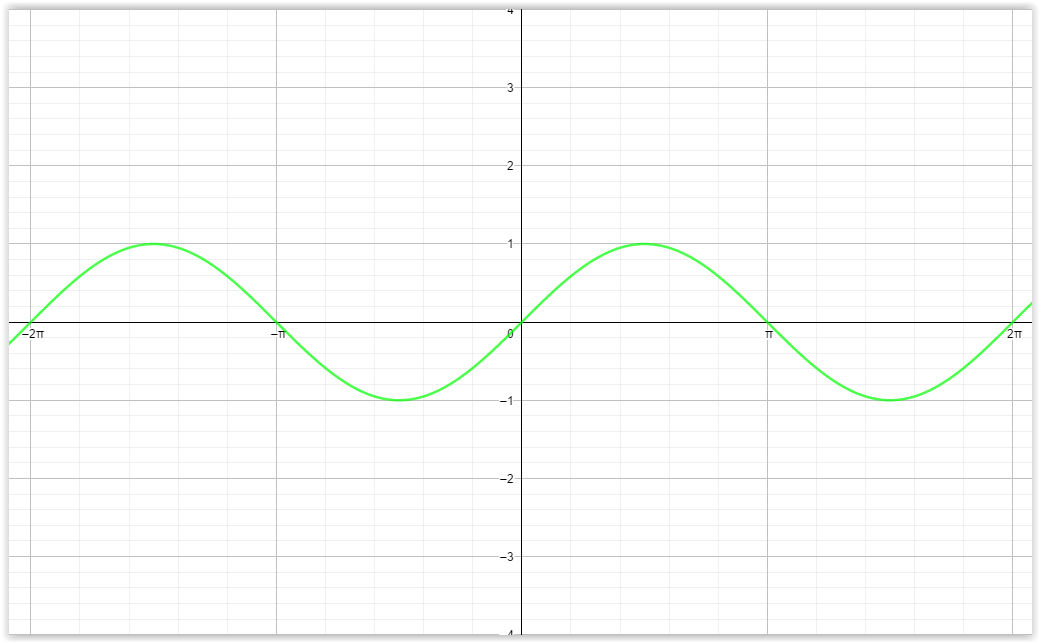
\includegraphics[width=0.9\linewidth]{./img/funktionen_sin.png}
		  \caption{Sinusfunktion}
		  \label{fig:funkt_sin}
		\end{minipage}%
		\begin{minipage}{.5\textwidth}
		  \centering
		  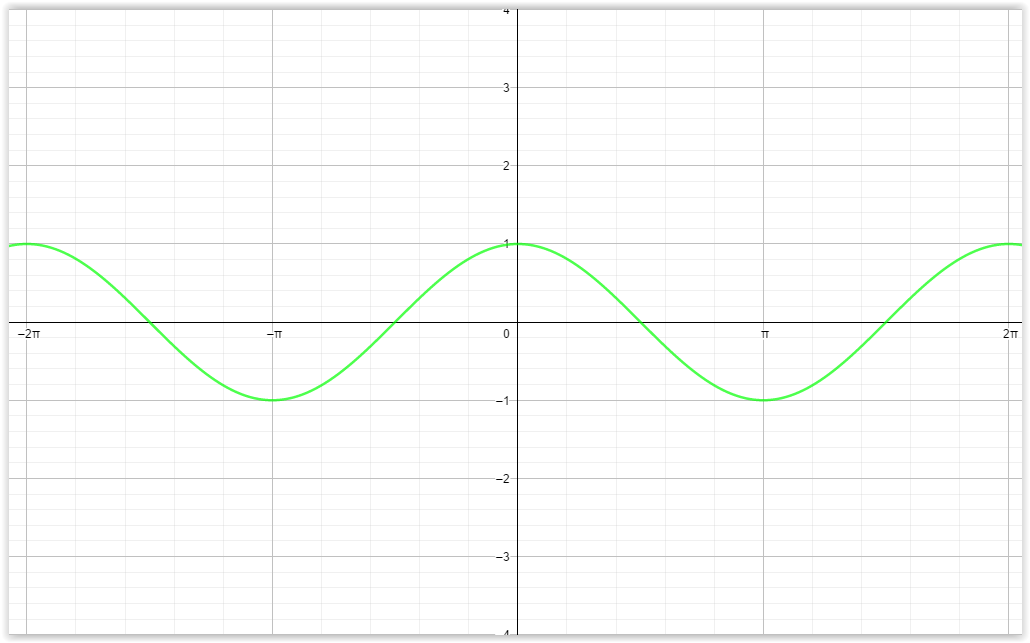
\includegraphics[width=0.9\linewidth]{./img/funktionen_cos.png}
		  \caption{Cosinusfunktion}
		  \label{fig:funkt_cos}
		\end{minipage}
		\end{figure}
		Es gelten folgende Zusammenhänge:\newline
		$\;$\newline
			\begin{tabular}{l | l}
				\tabitem $cos(x) = cos(-x)$ & 
				  \tabitem $e^z = e^{Re\lbrace z \rbrace} \left(cos(Im(z))+isin(Im(z))\right) \quad, z \in \C$\\
				\tabitem $-sin(x) = sin(-x)$ & \tabitem $sin(x) = \frac{1}{2i}\left(e^{ix}-e^{-ix}\right) \quad, x \in \R$\\
				\tabitem $cos(x+2 \pi) = cos(x)$ &  \tabitem $cos(x) = \frac{1}{2}\left(e^{ix}+e^{-ix}\right) \quad, x \in \R$\\
				\tabitem $sin(x+2\pi) = sin(x)$ & $\;$
		\end{tabular} \newline
		$\;$ \newline
		Weiterhin gilt:
		\begin{figure}[H]
		  \centering
		  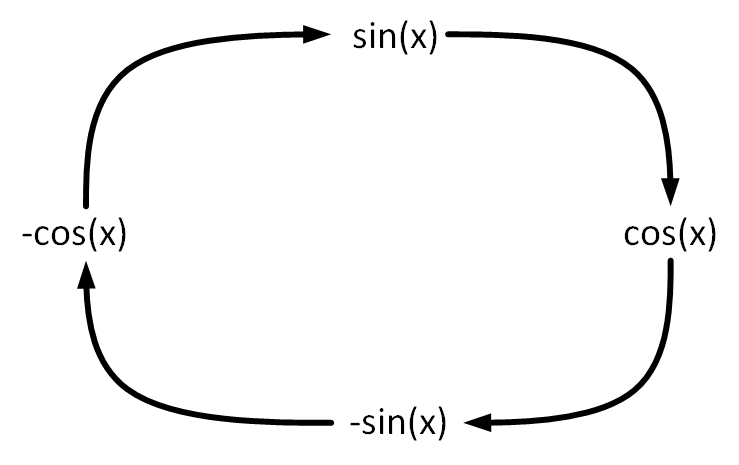
\includegraphics[width=0.35\linewidth]{./img/ableitungskreis.png}
		  \caption{Ableitungsregel}
		  \label{fig:funkt_trigo_abl_1}
		\end{figure}
		\subsubsubsection{Weitere trigonometrische Funktionen}
		\begin{equation}
		  tan(x) = \frac{sin(x)}{cos(x)}, \qquad  csc(x) = \frac{1}{sin(x)}, \qquad  cot(x),\; \dots
		\end{equation}
		\vspace{-0.5cm}
		\begin{figure}[H]
		  \centering
		  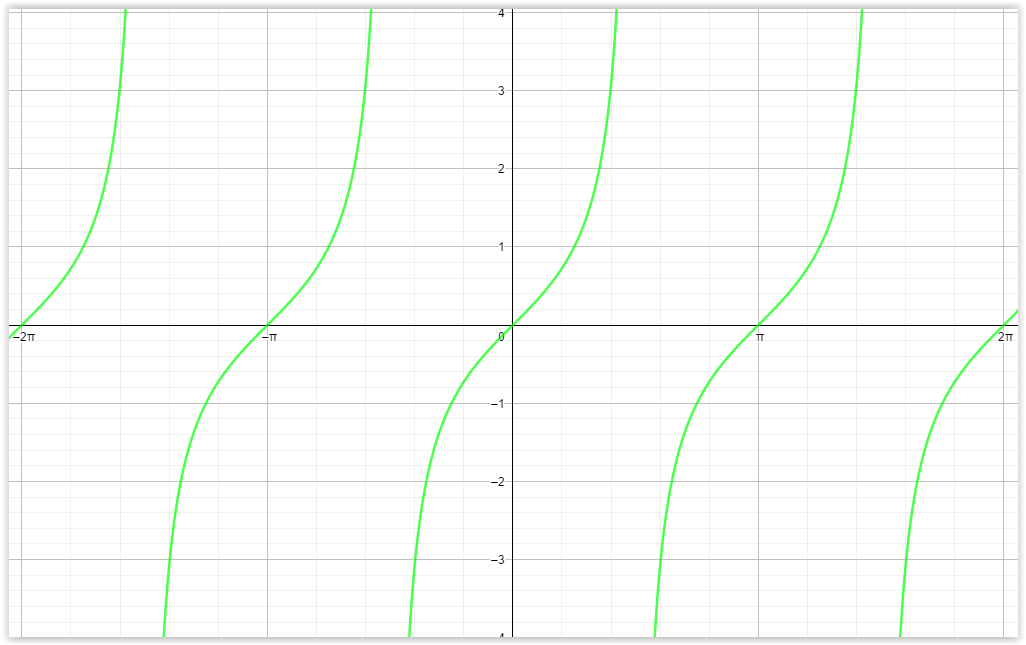
\includegraphics[width=0.5\linewidth]{./img/funktionen_tan.png}
		  \caption{$tan(x)$}
		  \label{fig:funkt_tan}
		\end{figure}
		\subsubsubsection{Hyperbolische Funktionen}
		\begin{align}
		  cosh(x) &= \frac{1}{2}\left( e^x + e^{-x}\right)\nonumber \\
		  sinh(x) &= \frac{1}{2}\left( e^x - e^{-x}\right)\nonumber \\
		  tanh(x) &= \frac{sinh(x)}{cosh(x)}\nonumber \\
		  sech,\;coth&,\; \dots ,\; etc.
		\end{align}
		\vspace{-0.7cm}  	  
	  \begin{figure}[H] 
		\centering
		\begin{minipage}{.5\textwidth}
		  \centering
		  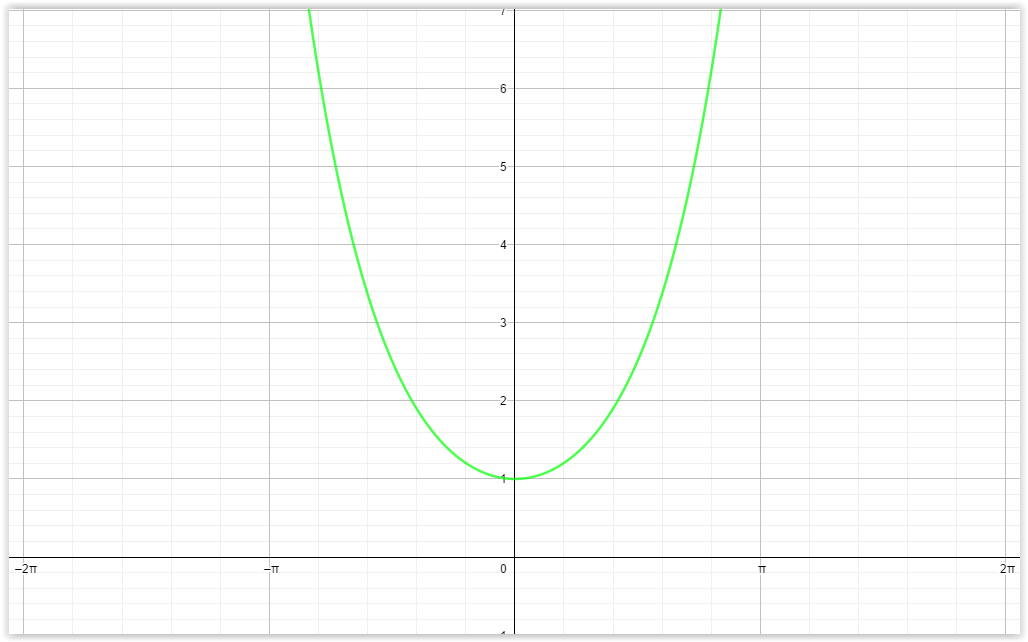
\includegraphics[width=0.8\linewidth]{./img/funktionen_cosh.png}
		  \caption{$y = cosh(x)$}
		  \label{fig:funkt_cosh}
		\end{minipage}%
		\begin{minipage}{.5\textwidth}
		  \centering
		  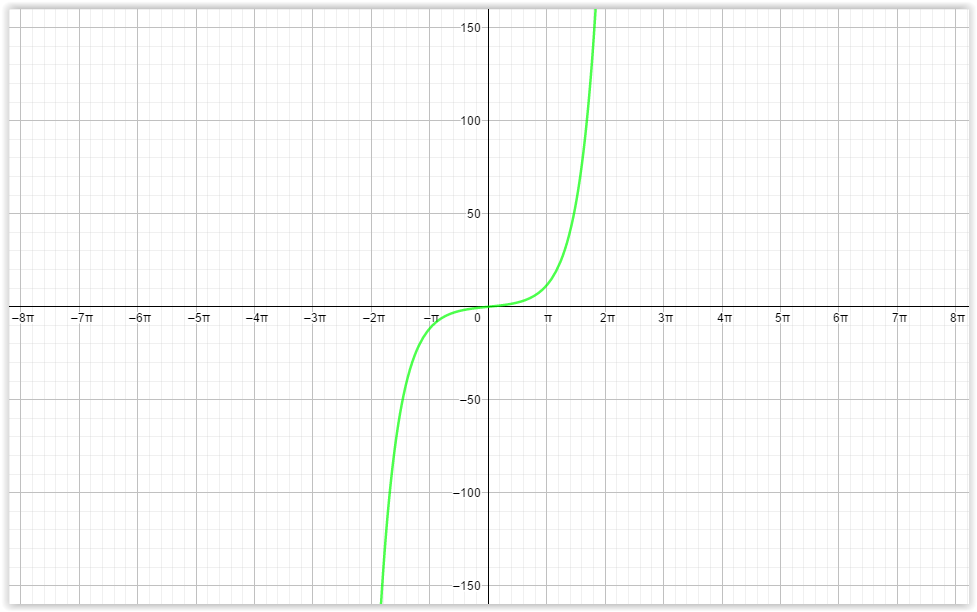
\includegraphics[width=0.8\linewidth]{./img/funktionen_sinh.png}
		  \caption{$y = sinh(x)$}
		  \label{fig:funkt_sinh}
		\end{minipage}
		\end{figure}
		\vspace{-0.5cm}
		\begin{figure}[H]
		  \centering
		  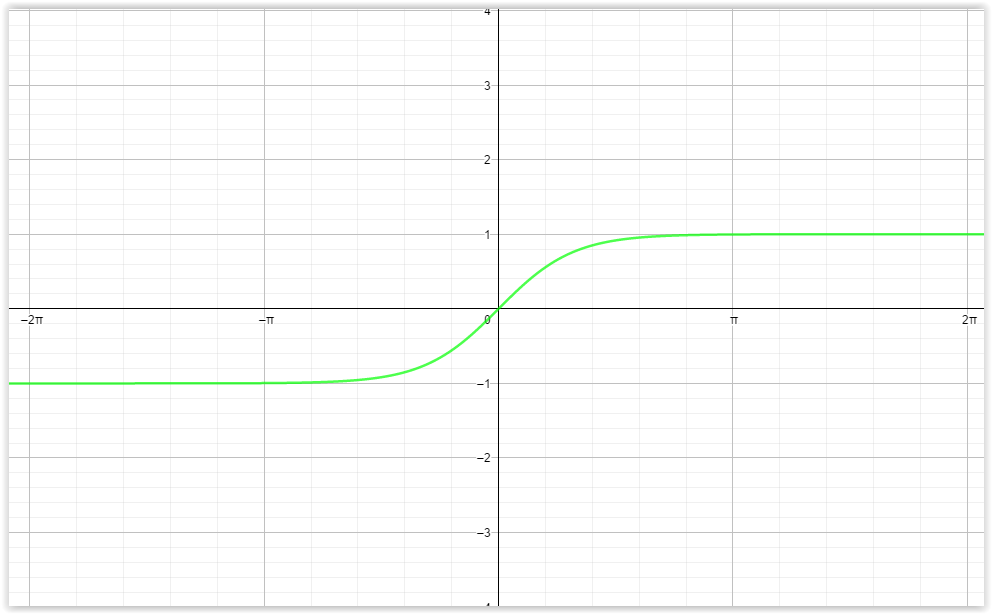
\includegraphics[width=0.4\linewidth]{./img/funktionen_tanh.png}
		  \caption{$y = tanh(x)$}
		  \label{fig:funkt_tanh}
		\end{figure}
		Es gelten folgende Identitäten:
		\begin{align}
		  \big(cosh(x)\big)' &= sinh(x) \\
		  \big(sinh(x)\big)' &= cosh(x) \\
		  cosh^2(x) - sinh^2(x) &= 1 \\
		  cos(z) &= \frac{1}{2}\left(e^{iz}+e^{iz}\right) = cosh(iz) \quad , z \in \C \\
		  sin(z) &= \frac{1}{2i}\left( e^{iz} - e^{iz}\right) = -isinh(/iz) \quad , z \in \C
		\end{align}
\newpage
